\section{Date: 2026-10-16}
\noindent \textbf{Series ID: BAMLCC8A015PYTRIV} 

\noindent This series is titled ICE BofA 15+ Year US Corporate Index Total Return Index Value and has a frequency of Daily, Close. The units are Index and the seasonal adjustment is Not Seasonally Adjusted.The observation start date is 2023-10-17 and the observation end date is 2026-10-15.The popularity of this series is 10. \\ 

\noindent \textbf{Series ID: CMATUR} 

\noindent This series is titled Unemployment Rate in Middle Atlantic division and has a frequency of Monthly. The units are Percent and the seasonal adjustment is Seasonally Adjusted.The observation start date is 1976-01-01 and the observation end date is 2026-08-01.The popularity of this series is 2. \\ 

\subsection{Raw Regression}
\noindent Regresses the two series against each other directly. A significant result here can come just as easily from both series sharing a long-run trend as from any real relationship.

\begin{center}
\begin{tabular}{lclc}
\toprule
\textbf{Dep. Variable:}                 & value\_fred\_CMATUR & \textbf{  R-squared:         } &     0.324   \\
\textbf{Model:}                         &         OLS         & \textbf{  Adj. R-squared:    } &     0.286   \\
\textbf{Method:}                        &    Least Squares    & \textbf{  F-statistic:       } &     8.618   \\
\textbf{Date:}                          &   Fri, 16 Oct 2026  & \textbf{  Prob (F-statistic):} &  0.00884    \\
\textbf{Time:}                          &       15:39:36      & \textbf{  Log-Likelihood:    } &    5.6116   \\
\textbf{No. Observations:}              &            20       & \textbf{  AIC:               } &    -7.223   \\
\textbf{Df Residuals:}                  &            18       & \textbf{  BIC:               } &    -5.232   \\
\textbf{Df Model:}                      &             1       & \textbf{                     } &             \\
\textbf{Covariance Type:}               &      nonrobust      & \textbf{                     } &             \\
\bottomrule
\end{tabular}
\begin{tabular}{lcccccc}
                                        & \textbf{coef} & \textbf{std err} & \textbf{t} & \textbf{P$> |$t$|$} & \textbf{[0.025} & \textbf{0.975]}  \\
\midrule
\textbf{const}                          &       1.8823  &        0.838     &     2.245  &         0.038        &        0.121    &        3.643     \\
\textbf{value\_fred\_BAMLCC8A015PYTRIV} &       0.0006  &        0.000     &     2.936  &         0.009        &        0.000    &        0.001     \\
\bottomrule
\end{tabular}
\begin{tabular}{lclc}
\textbf{Omnibus:}       &  1.277 & \textbf{  Durbin-Watson:     } &    0.475  \\
\textbf{Prob(Omnibus):} &  0.528 & \textbf{  Jarque-Bera (JB):  } &    1.121  \\
\textbf{Skew:}          &  0.506 & \textbf{  Prob(JB):          } &    0.571  \\
\textbf{Kurtosis:}      &  2.433 & \textbf{  Cond. No.          } & 8.54e+04  \\
\bottomrule
\end{tabular}
%\caption{OLS Regression Results}
\end{center}

Notes: \newline
 [1] Standard Errors assume that the covariance matrix of the errors is correctly specified. \newline
 [2] The condition number is large, 8.54e+04. This might indicate that there are \newline
 strong multicollinearity or other numerical problems.

\begin{figure}
\centering
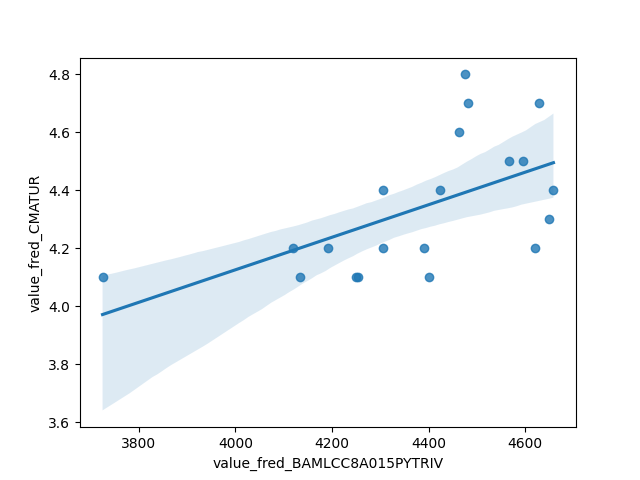
\includegraphics[scale = 0.9]{plots/plot_2026-10-16.png}
\caption{Raw Regression Plot for 2026-10-16}
\end{figure}
\newpage
\subsection{Detrended Regression}
\noindent Regresses the residuals of each series after removing its own linear time trend, so a shared trend can no longer drive the result on its own. A relationship that stays significant here is better evidence of a genuine link between the two series.

\begin{center}
\begin{tabular}{lclc}
\toprule
\textbf{Dep. Variable:}                            & value\_fred\_CMATUR\_detrended & \textbf{  R-squared:         } &     0.004   \\
\textbf{Model:}                                    &              OLS               & \textbf{  Adj. R-squared:    } &    -0.051   \\
\textbf{Method:}                                   &         Least Squares          & \textbf{  F-statistic:       } &   0.07620   \\
\textbf{Date:}                                     &        Fri, 16 Oct 2026        & \textbf{  Prob (F-statistic):} &    0.786    \\
\textbf{Time:}                                     &            15:39:36            & \textbf{  Log-Likelihood:    } &    9.8365   \\
\textbf{No. Observations:}                         &                 20             & \textbf{  AIC:               } &    -15.67   \\
\textbf{Df Residuals:}                             &                 18             & \textbf{  BIC:               } &    -13.68   \\
\textbf{Df Model:}                                 &                  1             & \textbf{                     } &             \\
\textbf{Covariance Type:}                          &           nonrobust            & \textbf{                     } &             \\
\bottomrule
\end{tabular}
\begin{tabular}{lcccccc}
                                                   & \textbf{coef} & \textbf{std err} & \textbf{t} & \textbf{P$> |$t$|$} & \textbf{[0.025} & \textbf{0.975]}  \\
\midrule
\textbf{const}                                     &   -2.495e-13  &        0.035     & -7.15e-12  &         1.000        &       -0.073    &        0.073     \\
\textbf{value\_fred\_BAMLCC8A015PYTRIV\_detrended} &   -7.098e-05  &        0.000     &    -0.276  &         0.786        &       -0.001    &        0.000     \\
\bottomrule
\end{tabular}
\begin{tabular}{lclc}
\textbf{Omnibus:}       &  2.989 & \textbf{  Durbin-Watson:     } &    0.437  \\
\textbf{Prob(Omnibus):} &  0.224 & \textbf{  Jarque-Bera (JB):  } &    1.399  \\
\textbf{Skew:}          &  0.594 & \textbf{  Prob(JB):          } &    0.497  \\
\textbf{Kurtosis:}      &  3.517 & \textbf{  Cond. No.          } &     136.  \\
\bottomrule
\end{tabular}
%\caption{OLS Regression Results}
\end{center}

Notes: \newline
 [1] Standard Errors assume that the covariance matrix of the errors is correctly specified.

\begin{figure}
\centering
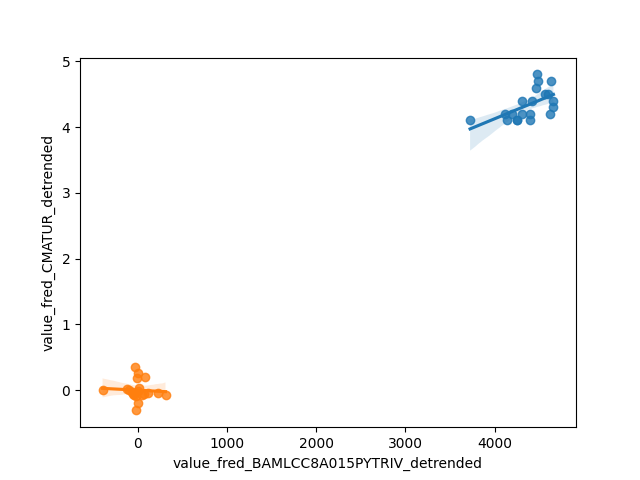
\includegraphics[scale = 0.9]{plots/plot_2026-10-16_detrended.png}
\caption{Detrended Regression Plot for 2026-10-16}
\end{figure}
\newpage
